\section{Final simulation results and discussions}
\label{sec:Simulations_And_Discutions}
This section presents simulations performed prior to the tapeout preparation, as no real measurements are available yet.
Also, will be carried out a comparison with an approximation of the 50 ohm EM termination which were applied at the CHIP shown in Appendix \ref{sec:Appendix} Figure \ref{fig:TapeoutChip}.\\
The design with ideal output ports is presented in the schematic of Figure~\ref{fig:Schematic_of_design_simulation_before_the_tapeout} in Section \ref{Analysis_combined_core}, whereas Figure~\ref{fig:Schematic_of_design_simulation_before_the_tapeout_measureAmplitude_PhaseImbalance} shows the corresponding imbalances.\\
The total supply current is \SI{29.194}{\meter\ampere} and the DC Power consumption is \SI{53}{\meter\watt}.\\
The requirements seems to be almost met as the amplitude imbalance is within \SI{\pm 0.15}{\decibel} while the phase imbalance is contained in a range of \SI{\pm 1.5}{\degree} with an offset in a band of frequencies between \SI{100}{\giga\hertz} and \SI{100}{\giga\hertz}.\\
%
\begin{figure}[hbt!]
    \centering
    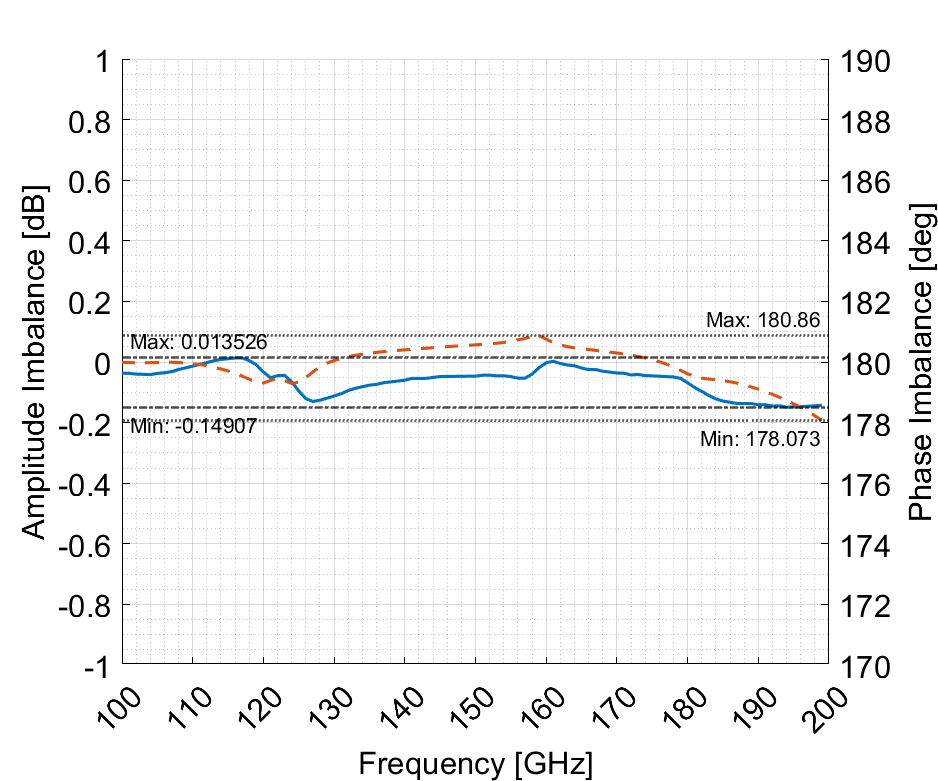
\includegraphics[width=0.75\linewidth]{Design_figures/Layout/TapeoutMeasurements/BalunDband_Design_SubmittedForTapeout_ExtractPar_SPprobe_MaxGain_Amplitude&PhaseImbalance}
    \caption{Simulation of the amplitude and phase imbalances of the final layout schematic with ideal \SI{50}{\ohm} loads.}
    \label{fig:Schematic_of_design_simulation_before_the_tapeout_measureAmplitude_PhaseImbalance}
\end{figure}
\\
The input and output S parameters are shown in Figure~\ref{fig:Schematic_of_design_simulation_before_the_tapeout_measureS11S22S33}, whereas the MaxGain and the forward transmission gains are illustrated in Figure~\ref{fig:Schematic_of_design_simulation_before_the_tapeout_measureMaxGain}. 
Within the D band, the MaxGain has an absolute peak of 14.5dB located around \SI{106}{\giga\hertz}, an absolute minimum value of almost 
\SI{7.67}{\decibel} at \SI{185}{\giga\hertz} and a local gain value of \SI{10.5}{\decibel} located around \SI{140}{\giga\hertz}.
It is evident that the trend of the parameter is not quite good looking.
The forward transmission gains $\mathrm{S}_{21}$ and $\mathrm{S}_{31}$ appears to be slightly more compact, although they do show the presence of losses in certain regions.\\
Ultimately, it would have been preferable for $\mathrm{S}_{11}$ and $\mathrm{S}_{33}$ to be less matched around \SI{106}{\giga\hertz} in favour of a more constant gain along the frequencies.
%
\begin{figure}[hbt!]
    \centering
    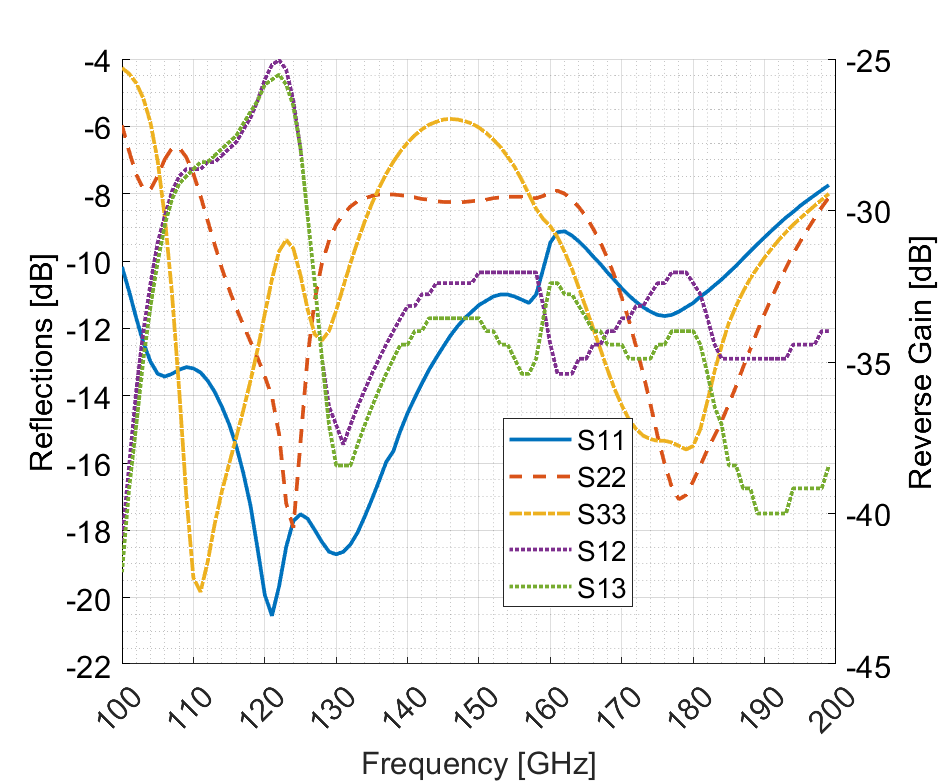
\includegraphics[width=0.75\linewidth]{Design_figures/Layout/TapeoutMeasurements/BalunDband_Design_SubmittedForTapeout_ExtractPar_SPprobe_MaxGain_Reflection&Reverse_S_parameters.png}
    \caption{Simulation of the reflection coefficients and reverse transmission gains of the final layout schematic with ideal \SI{50}{\ohm} loads.}
    \label{fig:Schematic_of_design_simulation_before_the_tapeout_measureS11S22S33}
\end{figure}
%
\begin{figure}[hbt!]
    \centering
    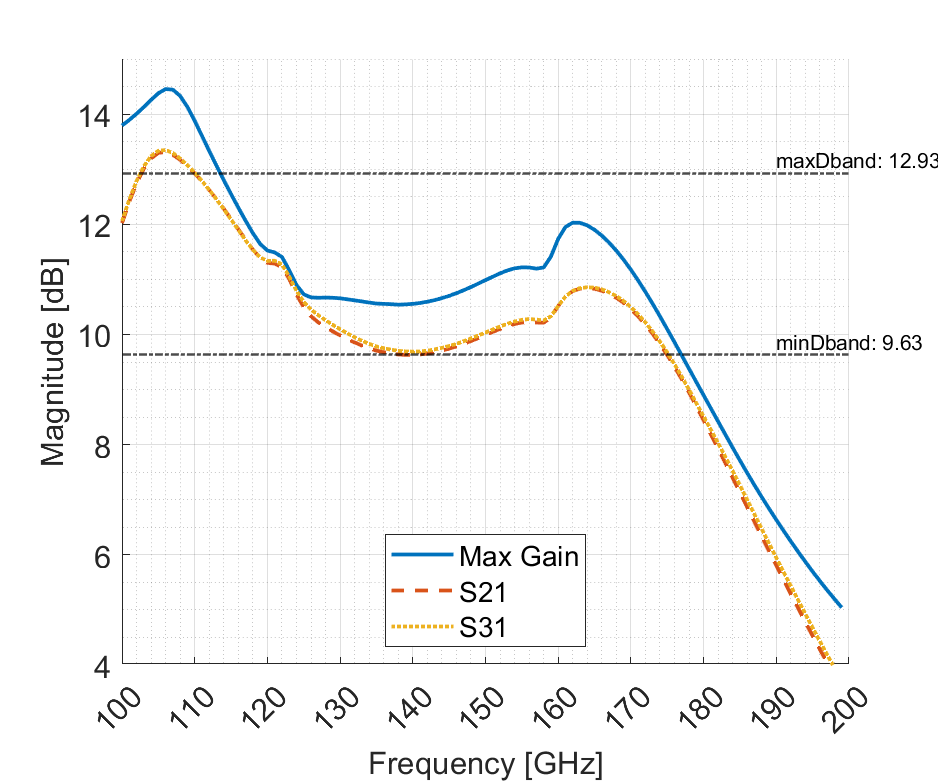
\includegraphics[width=0.75\linewidth]{Design_figures/Layout/TapeoutMeasurements/BalunDband_Design_SubmittedForTapeout_ExtractPar_SPprobe_MaxGain_Combined_MaxGain_S21_S31.png}
    \caption{Simulation of the MaxGain and forward transmission gain of the final layout schematic with ideal \SI{50}{\ohm} loads.}
    \label{fig:Schematic_of_design_simulation_before_the_tapeout_measureMaxGain}
\end{figure}
\clearpage
The Stability parameters are shown in Figure \ref{fig:BalunDband_Design_SubmittedForTapeout_ExtractPar_StabilityS21_K_Mu_Stability} and \ref{fig:BalunDband_Design_SubmittedForTapeout_ExtractPar_StabilityS31_K_Mu_Stability}.
\begin{figure}[hbt!]
    \centering
    \begin{subfigure}{0.48\textwidth}
        \centering
        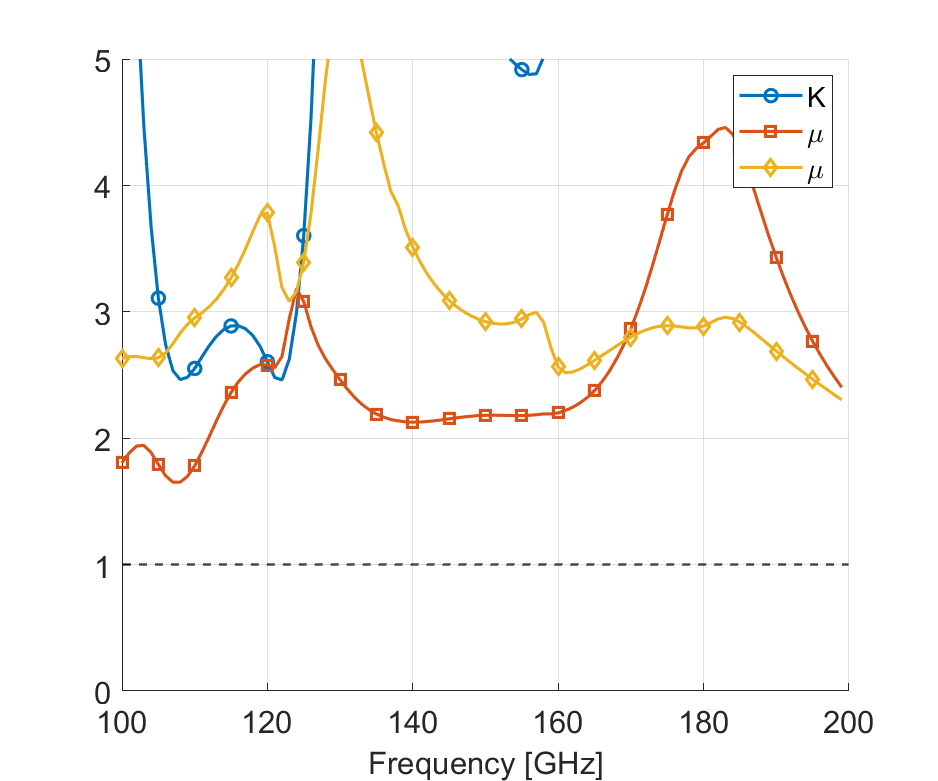
\includegraphics[width=\linewidth]{Design_figures/Layout/TapeoutMeasurements/BalunDband_Design_SubmittedForTapeout_ExtractPar_StabilityS21_K_Mu_Stability.png}
        \caption{}
    \label{fig:BalunDband_Design_SubmittedForTapeout_ExtractPar_StabilityS21_K_Mu_Stability}
    \end{subfigure}
    \hfill
    \begin{subfigure}{0.48\textwidth}
        \centering
        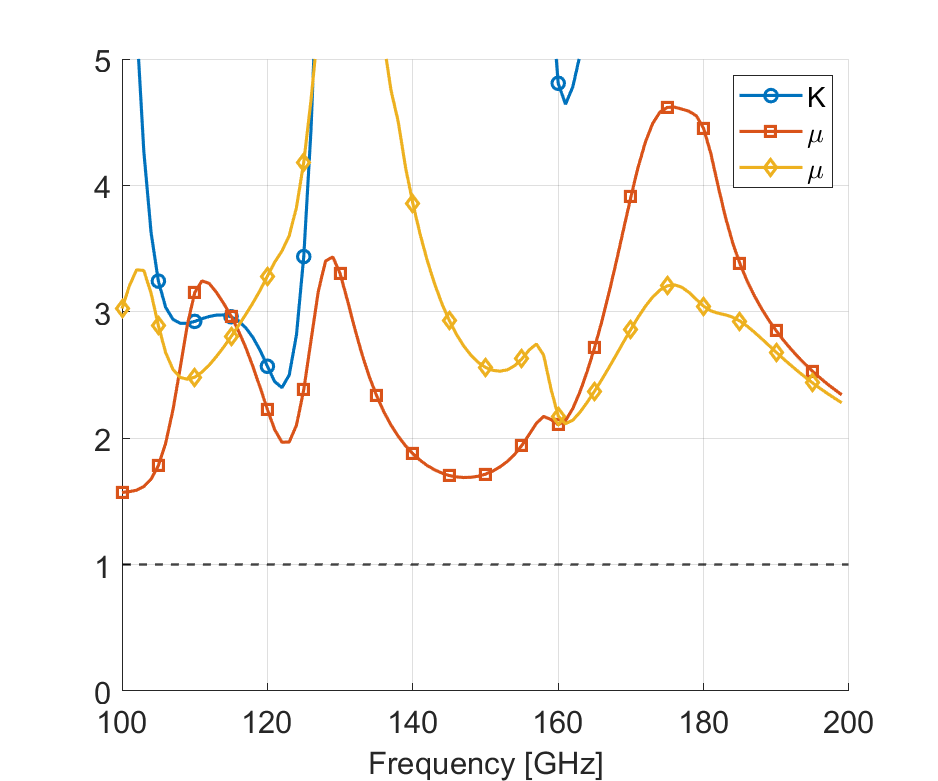
\includegraphics[width=\linewidth]{Design_figures/Layout/TapeoutMeasurements/BalunDband_Design_SubmittedForTapeout_ExtractPar_StabilityS31_K_Mu_Stability.png}
        \caption{}
    \label{fig:BalunDband_Design_SubmittedForTapeout_ExtractPar_StabilityS31_K_Mu_Stability}
    \end{subfigure}
    \caption{Simulated results and comparison of stability parameters of of the final layout schematic when (a) port 3 is terminated to a \SI{50}{\ohm} load, (b) port 2 is terminated to a \SI{50}{\ohm} load}
    \label{fig:placeholder}
\end{figure}
\paragraph{Approximation of the EM terminations applied in the CHIP}\mbox{}\\
Since no EM simulations of the complete circuit with EM load terminations were available at the end of the experience, the measurement plan of the design was developed based on a first approximation. 
In this approach, the load and the ground via were simulated separately and then connected to the original circuit as termination while the opposite output port was connected to an ideal \SI{50}{\ohm} termination from which the Respective S-parameter were extracted.
\begin{figure}[hbt!]
    \centering
    \begin{subfigure}{0.45\textwidth}
        \centering
        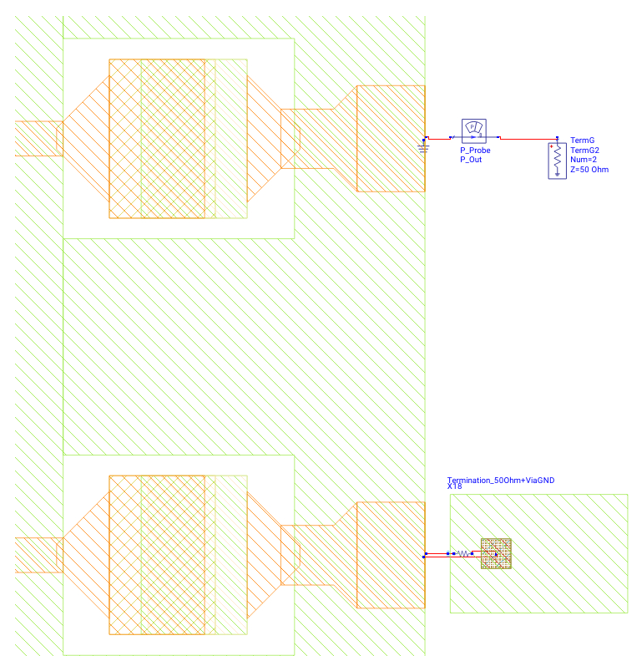
\includegraphics[width=0.90\linewidth]{Design_figures/Layout/TapeoutSchematics/EM_Bottomtermination.png}
        \caption{S21.BottomEMTerminated}
    \label{fig:placeholder}
    \end{subfigure}
    \hfill
    \begin{subfigure}{0.45\textwidth}
        \centering
        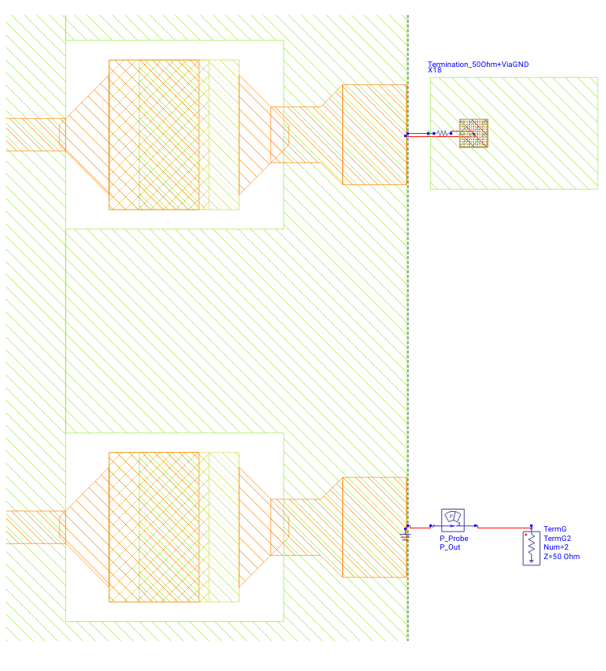
\includegraphics[width=0.90\linewidth]{Design_figures/Layout/TapeoutSchematics/EM_Toptermination.png}
        \caption{S21.TopEMTerminated}
    \label{fig:placeholder}
    \end{subfigure}
    \caption{Illustration of the EM load terminations adopted as a first approximation for the measurement plan.}
    \label{fig:placeholder}
\end{figure}
\\
The following paragraphs are based on the definitions given in the measurement plan. They also help the reader to understand which topic the description is referring to. The simulations consist of two phases named as:
\begin{itemize}
    \item "\textit{CalculatedS21.bottom EM terminated}" which is the effective $\mathrm{S}_{21}$ parameter. The output RF probe is connected to the top output port while bottom one is closed on a load within the layout;
    \item "\textit{CalculatedS21.top EM terminated}" which is referred to the old parameter $\mathrm{S}_{31}$. 
    The output RF probe is connected to the bottom output port while top one is closed on a load within the layout.
\end{itemize}
The plotted parameters are defined as:
\begin{align*}
\text{AmplitudeImbalanceEMTerminated} &=\\
\text{CalculatedS21.bottomEM (dB)} &- \text{CalculatedS21.topEM (dB);}\\
\text{PhaseImbalanceEMTerminated} &= \\
\text{phase(CalculatedS21.bottomEM)} &- \text{phase(CalculatedS21.topEM)};
\end{align*}

\begin{comment}
    while the y axis labeled as "AmplitudeImbalance" and "Phase Imbalance" are referred to the plots terminated with ideal loads in Figure\ref{fig:Schematic_of_design_simulation_before_the_tapeout_measureAmplitude_PhaseImbalance}.\\
\end{comment}
Also, simulations of the IP1dB and OP1dB have been carried out and are illustrated in the next figures.

\paragraph{CalculatedS21.bottom EM terminated}\mbox{\\}

The forward gain is displayed in Figure \ref{fig:_MeasureS21_ExtractPar_SPprobe_MaxGain_S21_BottomTerminated} and the reflection coefficients in Figure \ref{fig:MeasureS21_ExtractPar_SPprobe_MaxGain_S22&S11_BottomTerminated}.
\begin{figure}[H]
    \centering
    \begin{subfigure}{0.49\textwidth}
        \centering
        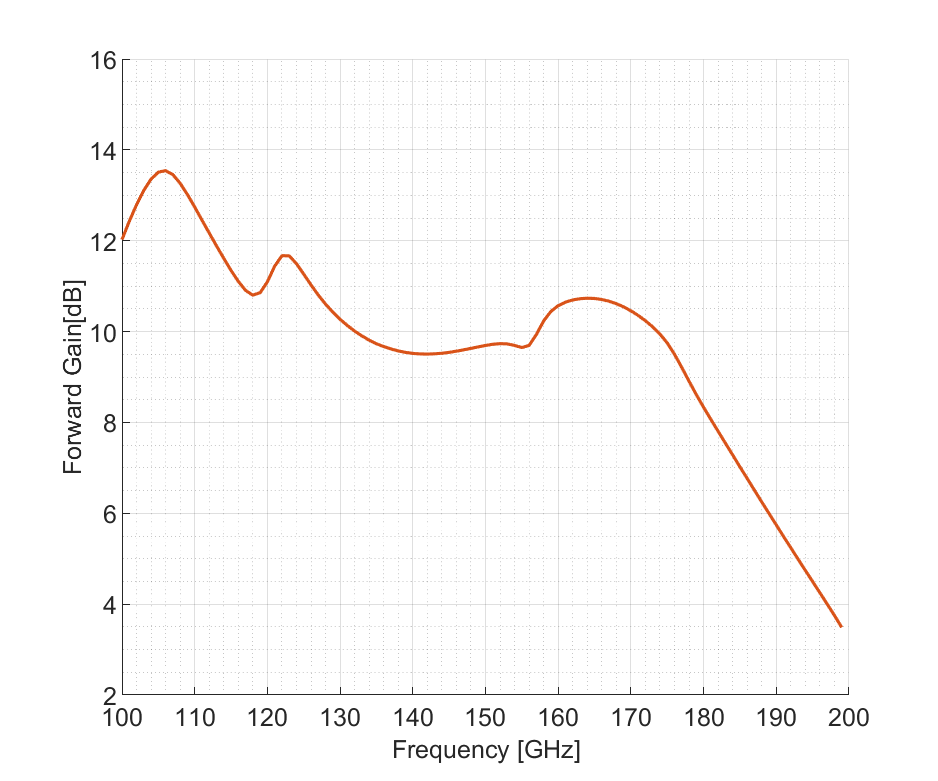
\includegraphics[width=\linewidth]{Design_figures/Layout/TapeoutMeasurements/BalunDband_Design_SubmittedForTapeout_MeasureS21_ExtractPar_SPprobe_MaxGain_S21_BottomTerminated.png}
        \caption{}
        \label{fig:_MeasureS21_ExtractPar_SPprobe_MaxGain_S21_BottomTerminated}
    \end{subfigure}
    \hfill
    \begin{subfigure}{0.49\textwidth}
        \centering
        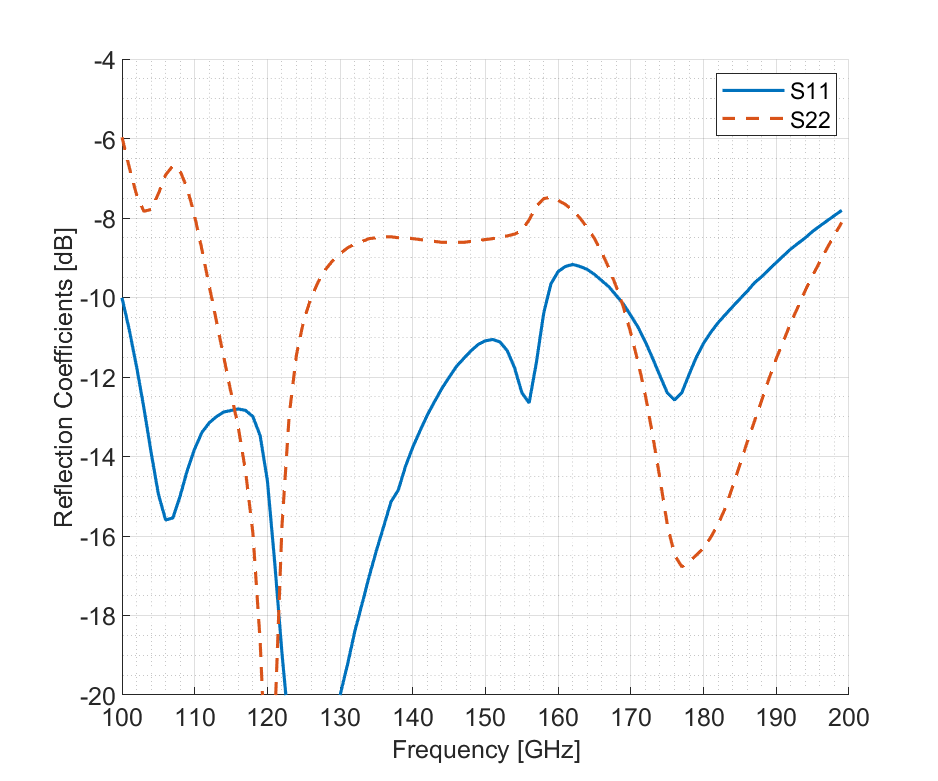
\includegraphics[width=\linewidth]{Design_figures/Layout/TapeoutMeasurements/BalunDband_Design_SubmittedForTapeout_MeasureS21_ExtractPar_SPprobe_MaxGain_S22&S11_BottomTerminated.png}
        \caption{}
        \label{fig:MeasureS21_ExtractPar_SPprobe_MaxGain_S22&S11_BottomTerminated}
    \end{subfigure}
    \caption{Simulation of (a) the forward transmission gain and (b) the reflection coefficient at output Port2 when Port3 is EM-terminated (S21.BottomEMTerminated).}
    \label{fig:placeholder}
\end{figure}

\begin{figure}[H]
    \centering
    % Colonna di sinistra
    \begin{minipage}[t]{0.8\textwidth}
        \centering
        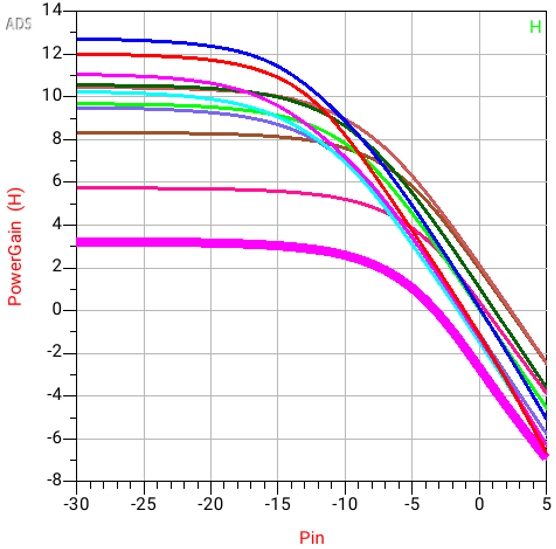
\includegraphics[width=0.75\linewidth]{Design_figures/Layout/TapeoutMeasurements/MeasureS21_IP1dB.png}\\[1em]
        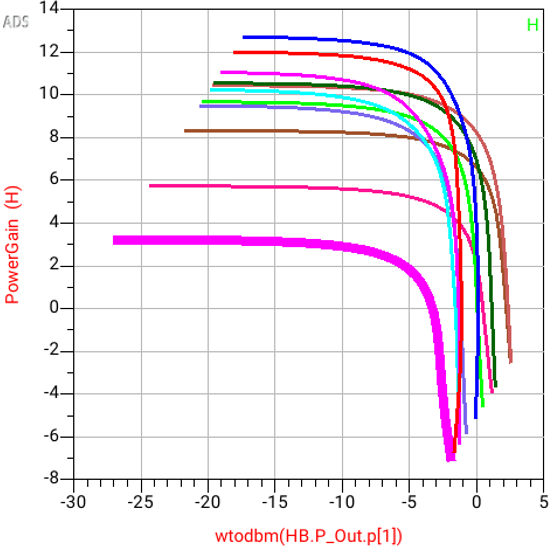
\includegraphics[width=0.75\linewidth]{Design_figures/Layout/TapeoutMeasurements/MeasureS21_OP1dB.png}
    \end{minipage}
    \hspace{-1cm}
    % Figura a destra centrata verticalmente
    \begin{minipage}[c]{0.2\textwidth}
        \centering
        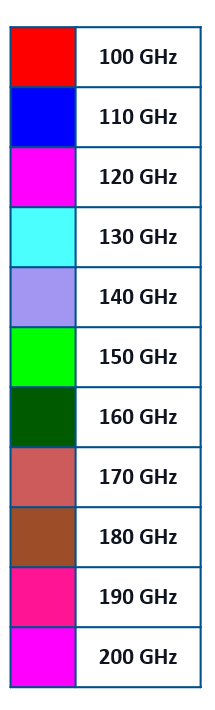
\includegraphics[width=0.75\linewidth]{Design_figures/Layout/TapeoutMeasurements/Scale.png}
    \end{minipage}
    \caption{Simulation of the IP1dB (top) and OP1dB (bottom) at the output Port2 when the Port3 is EM-terminated (S21.BottomEMTerminated).}
    \label{fig:powerGain_measuresS21}
\end{figure}
%
Figure \ref{fig:powerGain_measuresS21} shows, in the top, the output power gain versus the input power and, in the bottom, the output power gain versus the output power. Both were simulated at intervals of \SI{10}{\giga\hertz} between \SI{100}{\giga\hertz} and \SI{200}{\giga\hertz}.\
In the top plot, at \SI{100}{\giga\hertz}, the amplifier exhibits a small-signal gain of \SI{12}{\decibel}. The IP1dB, which corresponds to the input power at which the output decreases by \SI{1}{\decibel} and enters in compression, is about \SI{-15}{\decibel\milli\watt}.
As the frequency increases to \SI{110}{\giga\hertz} (\SI{120}{\giga\hertz}), an increase (decrease) in the output power to \SI{13}{\decibel} (\SI{11}{\decibel}) and a IP1dB of \SI{-17}{\decibel} (\SI{-12.5}{\decibel\milli\watt}) can be observed.
Beyond \SI{130}{\giga\hertz} and up to \SI{170}{\giga\hertz}, the output power mostly flattens but a decreasing trend can still be noticed. in this range the output power provides values between \SI{10.5}{\decibel} and \SI{9.5}{\decibel} with the corresponding IP1dB values between \SI{-10}{\decibel\milli\watt} and \SI{-12}{\decibel\milli\watt}.\\
%
At \SI{180}{\giga\hertz}, the output power increases one last time at \SI{10.3}{\decibel} (as the power at \SI{160}{\giga\hertz}), with the corresponding IP1dB at \SI{-9}{\decibel\milli\watt}.
above the \SI{170}{\giga\hertz}, the frequency roll-off starts to become important. At \SI{190}{\giga\hertz}, the output power decreases to \SI{5.8}{\decibel}, with IP1dB at \SI{-3}{\decibel\milli\watt}.
The same analysis was repeated for several frequencies to evaluate the frequency dependence of the compression behavior.\\

In the bottom plot of Figure~\ref{fig:powerGain_measuresS21}, at \SI{100}{\giga\hertz}, the output power is the same as described previously, but the OP1dB, which corresponds to the output power at which the fundamental component of the output decreases by \SI{1}{\decibel} and enters compression, is about \SI{-4}{\decibel\milli\watt}.
As the frequency increases to \SI{110}{\giga\hertz} (\SI{120}{\giga\hertz}), an OP1dB of \SI{-4}{\decibel\milli\watt} (\SI{-7}{\decibel\milli\watt}) can be observed.
Beyond \SI{130}{\giga\hertz} and up to \SI{170}{\giga\hertz}, the corresponding OP1dB values are between \SI{-6}{\decibel\milli\watt} and \SI{-1}{\decibel\milli\watt}.
At \SI{180}{\giga\hertz}, the corresponding OP1dB is \SI{-1}{\decibel\milli\watt}, and at \SI{190}{\giga\hertz}, it is \SI{-2.5}{\decibel\milli\watt}.
\begin{comment}
    \begin{table}[h]
\centering
\begin{tabular}{|c|c c c|}
\hline
Frequency (GHz) & PowerGain (dB) & IP1dB (dBm) & OP1dB (dBm) \\
\hline
100  &  &  &  \\
\hline
110 &  &  &  \\
120 &  &  &  \\
\hline
130 &  &  &  \\
140 &  &  &  \\
150 &  &  &  \\
160 &  &  &  \\
170 &  &  &  \\
180 &  &  &  \\
\hline
190 &  &  &  \\
200 &  &  &  \\
\hline
\end{tabular}
\caption{PowerGain, IP1dB, OP1dB with port 3 is connected to an EM Termination}
\label{tab:performance}
\end{table}
\end{comment}

%\cleardoublepage
\paragraph{CalculatedS21.top EM terminated}
The forward gain is displayed in Figure \ref{fig:MeasureS31_ExtractPar_SPprobe_MaxGain_S21_TopTerminated} and the reflection coefficients in Figure \ref{fig:MeasureS31_ExtractPar_SPprobe_MaxGain_S22&S11_TopTerminated}.
\begin{center}
\begin{figure}[H]
    \centering
    \begin{subfigure}{0.49\textwidth}
        \centering
        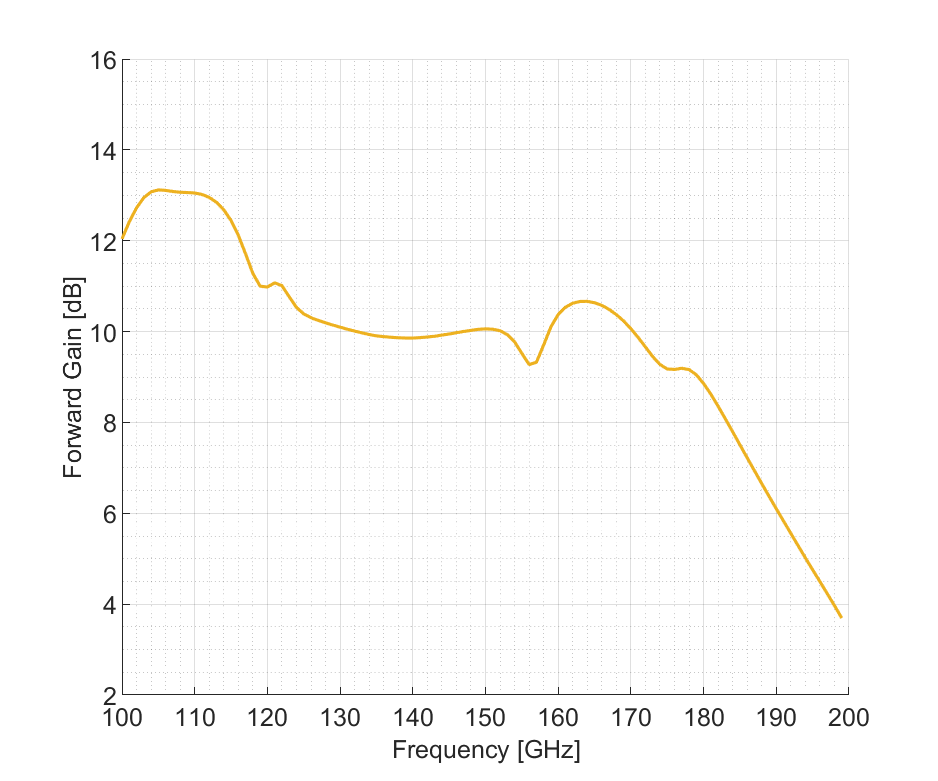
\includegraphics[width=\linewidth]{Design_figures/Layout/TapeoutMeasurements/BalunDband_Design_SubmittedForTapeout_MeasureS31_ExtractPar_SPprobe_MaxGain_S21_TopTerminated.png}
        \caption{}
        \label{fig:MeasureS31_ExtractPar_SPprobe_MaxGain_S21_TopTerminated}
    \end{subfigure}
    \hfill
    \begin{subfigure}{0.49\textwidth}
        \centering
        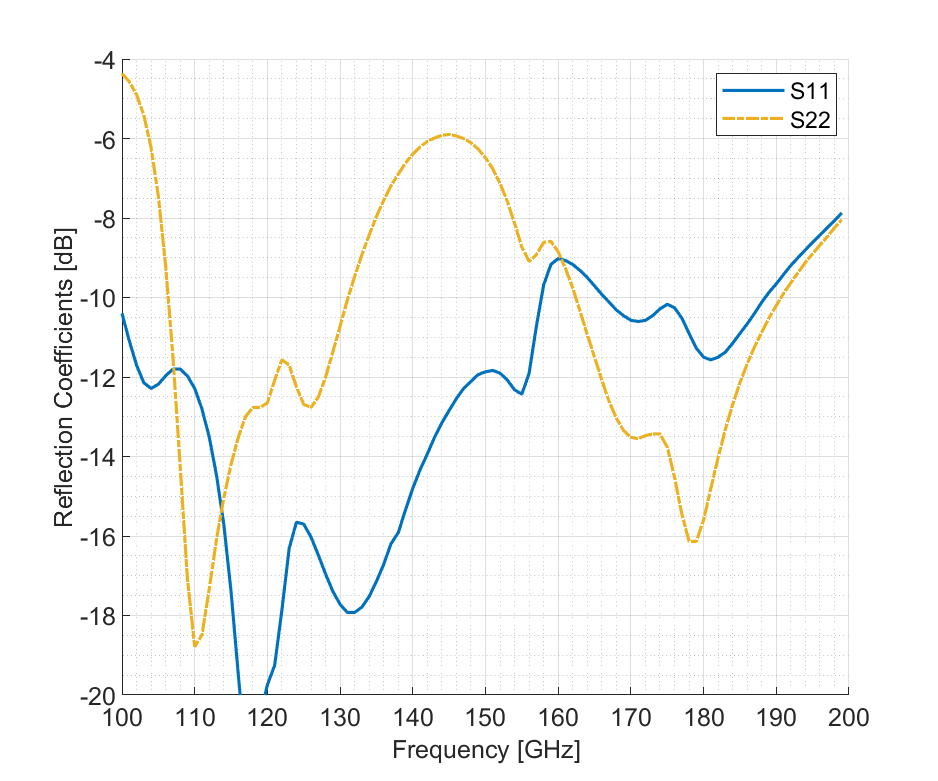
\includegraphics[width=\linewidth]{Design_figures/Layout/TapeoutMeasurements/BalunDband_Design_SubmittedForTapeout_MeasureS31_ExtractPar_SPprobe_MaxGain_S22&S11_TopTerminated.png}
        \caption{}
        \label{fig:MeasureS31_ExtractPar_SPprobe_MaxGain_S22&S11_TopTerminated}
    \end{subfigure}
    \caption{Simulation of (a) the forward transmission gain and (b) the reflection coefficient at output Port3 when Port2 is EM-terminated (S21.TopEMTerminated).}
    \label{fig:placeholder}
\end{figure}
\end{center}
The IP1dB and OP1dB results, shown in Figure~\ref{fig:powerGain_measuresS31}, agree with the formula $\mathrm{OP1dB} = \mathrm{IP1dB} + \mathrm{PowerGain}$. Since the previous values were estimated by eye, some approximation is present. However, it is still possible to observe that the circuit behaves linearly, as the gain and the output power are related to each other.
\begin{comment}
    \begin{table}[h]
\centering
\begin{tabular}{|c|c c c|}
\hline
Frequency (GHz) & PowerGain (dB) & IP1dB (dBm) & OP1dB (dBm) \\
\hline
100  &  &  &  \\
\hline
110 &  &  &  \\
120 &  &  &  \\
\hline
130 &  &  &  \\
140 &  &  &  \\
150 &  &  &  \\
160 &  &  &  \\
170 &  &  &  \\
180 &  &  &  \\
\hline
190 &  &  &  \\
200 &  &  &  \\
\hline
\end{tabular}
\caption{PowerGain, IP1dB, OP1dB with port 3 is connected to an EM Termination}
\label{tab:performance}
\end{table}
\end{comment}

\begin{center}
\begin{figure}[H]
    \centering
    % Colonna di sinistra
    \begin{minipage}[t]{0.79\textwidth}
        \centering
        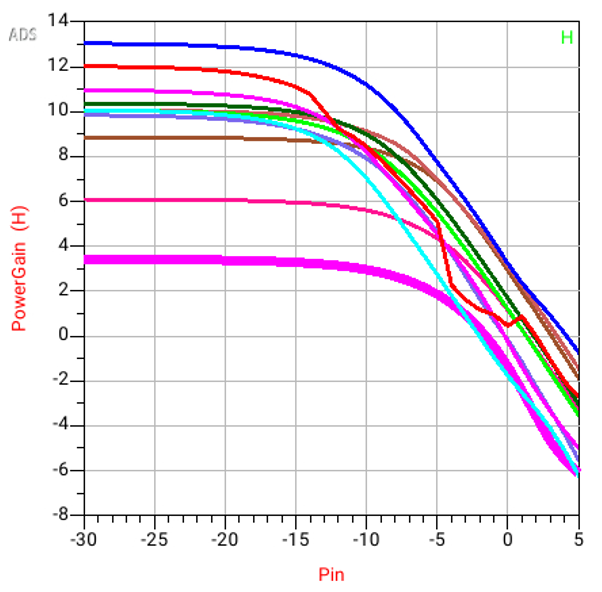
\includegraphics[width=0.75\linewidth]{Design_figures/Layout/TapeoutMeasurements/MeasureS31_IP1dB.png}\\[1em]
        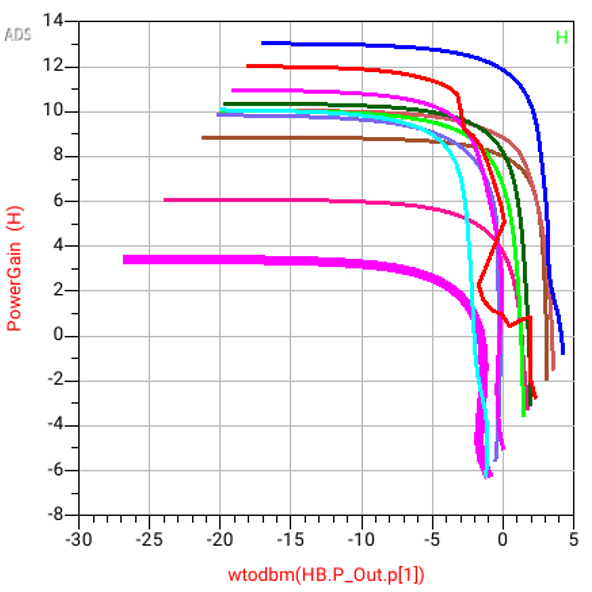
\includegraphics[width=0.75\linewidth]{Design_figures/Layout/TapeoutMeasurements/MeasureS31_OP1dB.png}
    \end{minipage}
    \hspace{-1cm}
    % Figura a destra centrata verticalmente
    \begin{minipage}[c]{0.2\textwidth}
        \centering
        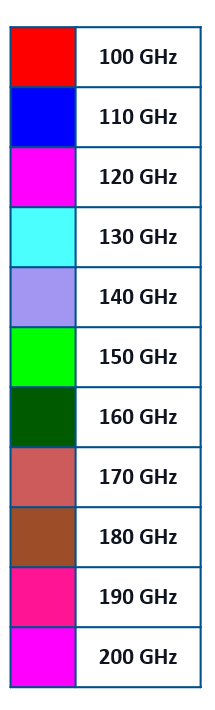
\includegraphics[width=0.75\linewidth]{Design_figures/Layout/TapeoutMeasurements/Scale.png}
    \end{minipage}
    \caption{Simulation of the IP1dB (top) and OP1dB (bottom) at the output Port3 when the Port2 is EM-terminated (S21.TopEMTerminated).}
    \label{fig:powerGain_measuresS31}
\end{figure}
\end{center}
%
\clearpage
\paragraph{Simulated imbalances with EM terminations}\mbox{}\\
The results in Figure \ref{fig:EM_Terminations_measurements} show a great discrepancy from the expected values:
The Amplitude imbalance is now within \SI{\pm 1.2}{\decibel} meanwhile the phase imbalance is \SI{\pm 7}{\degree}.
\begin{figure}[hbt!]
    \centering
    \begin{subfigure}{0.49\textwidth}
        \centering
        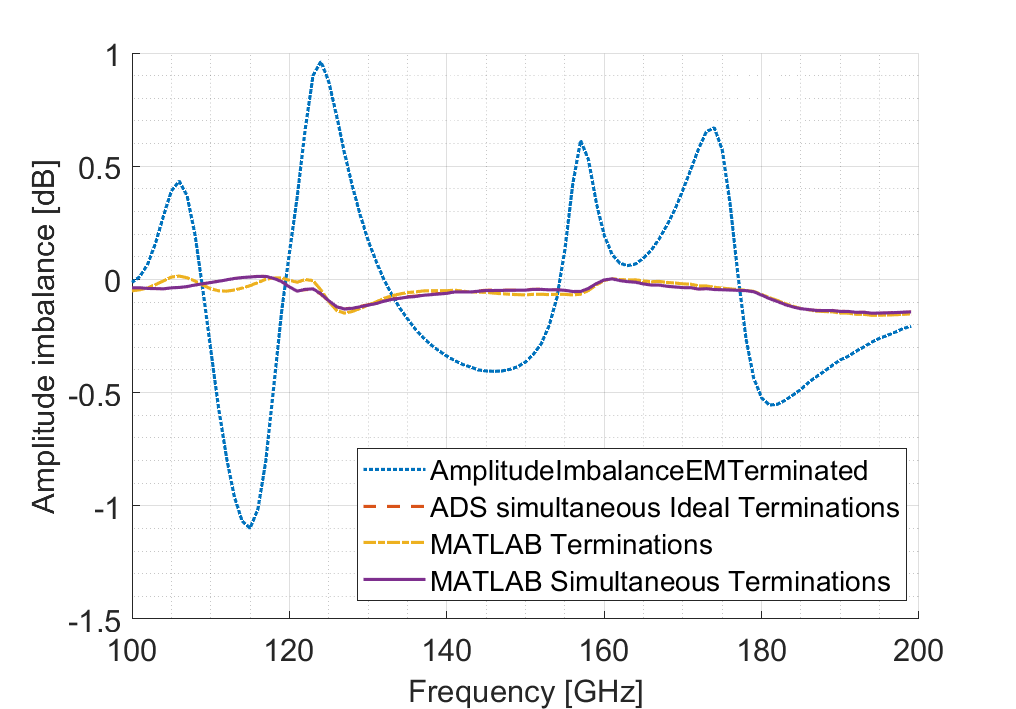
\includegraphics[width=\linewidth]{Design_figures/Layout/TapeoutMeasurements/FinalComparationAmplitudeImbalance_MatlabTermination.png}
        \caption{}
        \label{}
    \end{subfigure}
    \hfill
    \begin{subfigure}{0.49\textwidth}
        \centering
        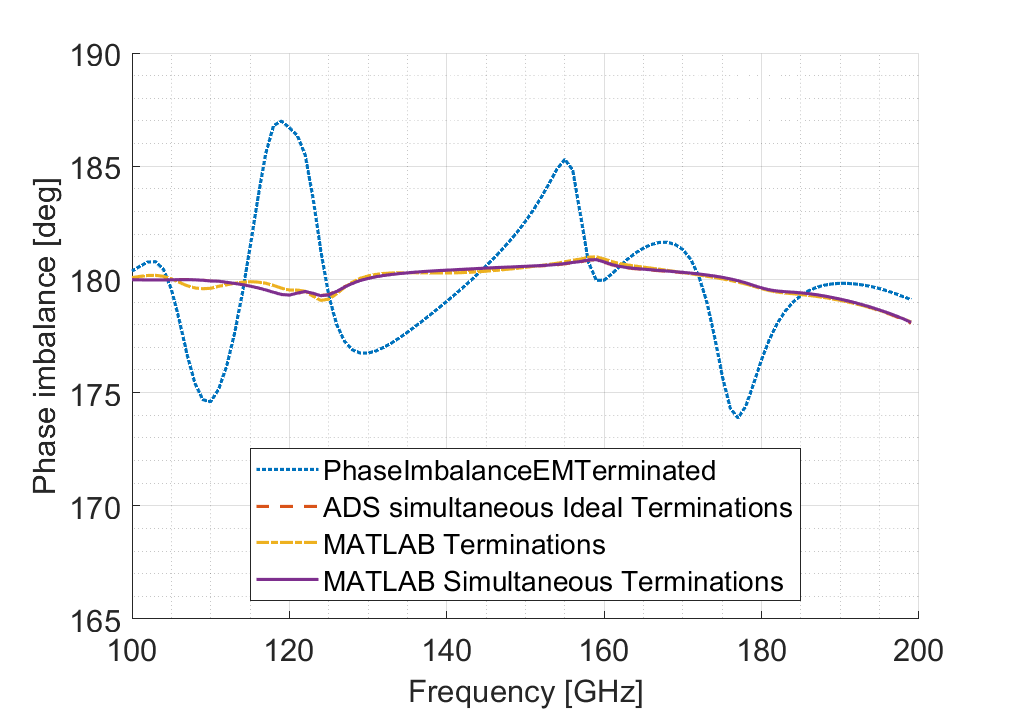
\includegraphics[width=\linewidth]{Design_figures/Layout/TapeoutMeasurements/FinalComparationPhaseImbalance_MatlabTermination.png}
        \caption{}
        \label{}
    \end{subfigure}
    \caption{Simulation and comparison between ADS data and virtual load variations in MATLAB for (a) amplitude imbalance and (b) phase imbalance}
    \label{fig:EM_Terminations_measurements}
\end{figure}

This deviation can be attributed to the fact that the S-parameters were not calculated with simultaneous terminations at the output ports, which resulted in the creation of mixed-mode conversion terms that would otherwise be close to zero.
\\
A simulation of this behaviour was found to be unsuccessful on MATLAB: The analysis was performed using the CSV datas retrieved from the design in Figure \ref{fig:Schematic_of_design_simulation_before_the_tapeout} whose parameters were taken with ideal simultaneous \SI{50}{\ohm} terminations, then the impedance value was changed to a value given by the EM simulation of the layout termination, Figure \ref{fig:EM_load_Terminations}, which, for semplicity has been supposed to be of value $(49-j2)\,\si{\ohm}$ and constant along all the D band. The resulting magnitude variation, showed in Figure \ref{fig:EM_Terminations_measurements}, was found to be negligible, presumably because the adopted S-parameters represent a screenshot of the circuit under symmetric loading conditions and thus, a mathematical variation does not recreate the real behavior happening on ADS.

\begin{comment}
    In fact, by not doing so, the S parameters measured at port 2 were affected only by the port 3 termination, giving way different results respect the S parameters measure at port 3 when port 2 was closed.

in this context Two type to simulations were done to verify and match the measurements performed in ADS, and to verify the results with simultaneous terminations.

The analysis was performed using the CSV datas retrieved from the design in Figure \ref{fig:Schematic_of_design_simulation_before_the_tapeout} whose parameters were taken with ideal \SI{50}{\ohm} terminations. By using MATLAB, a virtual variation of the load was performed. The load impedance was changed from the ideal \SI{50}{\ohm} to a value given by the EM simulation of the layout termination (\ref{fig:EM_load_Terminations}) which, for semplicity has been supposed to be with value 48-j2 and constant along all the D band. The magnitude variation was found to be negligible, indicating that the cause might be investigated somewhere else.

Maybe differential and common mode impedances? 
\end{comment}

\begin{comment}
     
were most probably interations within the ADS environment with the addition of the circuit not being completly symmetrical anymore.
This behaviour cannot properly be replicated in MATLAB as the retrieved S parameters refers to black box known to be a symmetric circuit. A so virtual termination on one output port does not affect other parameters in the same way as ads.
The variation of Z0, however, shown an interesting result. Changing Z0 from the standard value to 75-j50 creates almost the same effect, making  
believe that in the presence of asymmetric EM termination, the ideal Z0 changes to something different.
\end{comment}
\begin{comment}
was most probably on the other hand of the connection.
%
\begin{figure}[H]
    \centering
    \includegraphics[width=0.6\linewidth]{Design_figures/Layout/TapeoutMeasurements/IMPEDENZE_IN_USCITA.png}
    \caption{Caption}
    \label{fig:Z0_output}
\end{figure}

it is possible to see the resultant impedances seen from $S_{22}$ and $S_{33}$ ports by taking their respective plots in figure XX and applying the standard conversion formulas from S to Z parameters. the values acquired are shown in figure XX and illustrates that the impedances are not close to 50 ohm: a reflection coefficient $S_{ii}$ of -7.5 at 150GHz creates an resitance $Z_{ii} = 50*\frac{50-0.42}{1+0.42}=123 \Omega$. Taking this into account, if the transmission impedance defined in MATLAB is changed from 50 ohm to a value derived from $S_{11}$ and $S_{22}$, for example $Z=75-j50$), and if the measured value of the termination $Z_L$ is used,  the result of the imbalances starts to become very similar in both magnitude and behavior.
\begin{figure}[hbt]
    \centering
    \begin{subfigure}{0.48\textwidth}
        \centering
        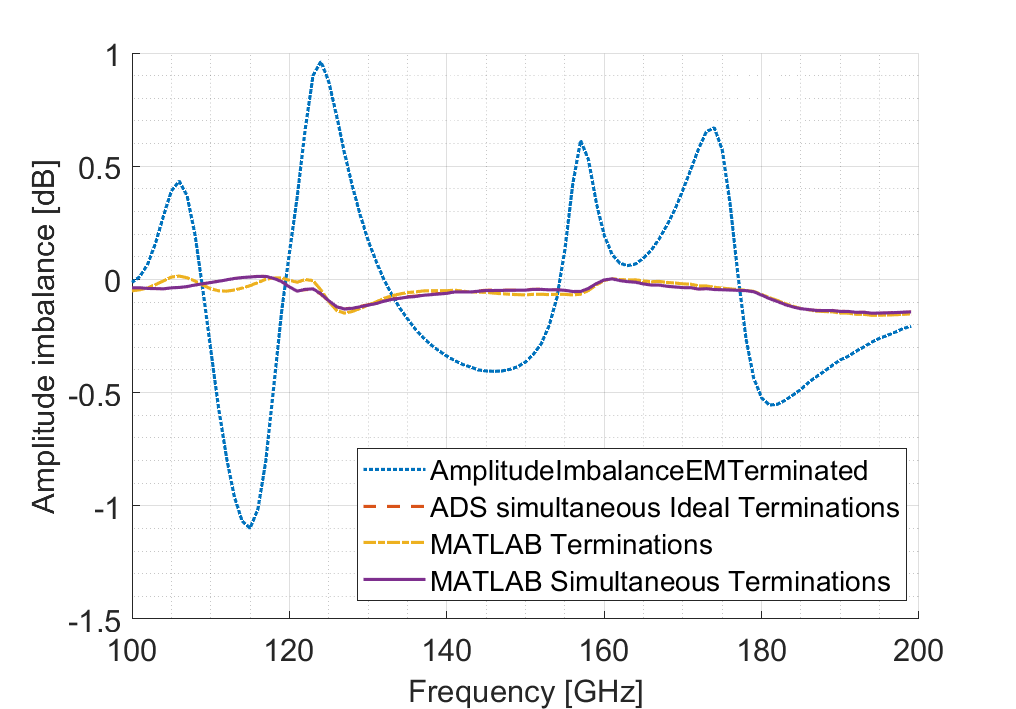
\includegraphics[width=\linewidth]{Design_figures/Layout/TapeoutMeasurements/FinalComparationAmplitudeImbalance_MatlabTermination.png}
    \end{subfigure}
    \hfill
    \begin{subfigure}{0.48\textwidth}
        \centering
        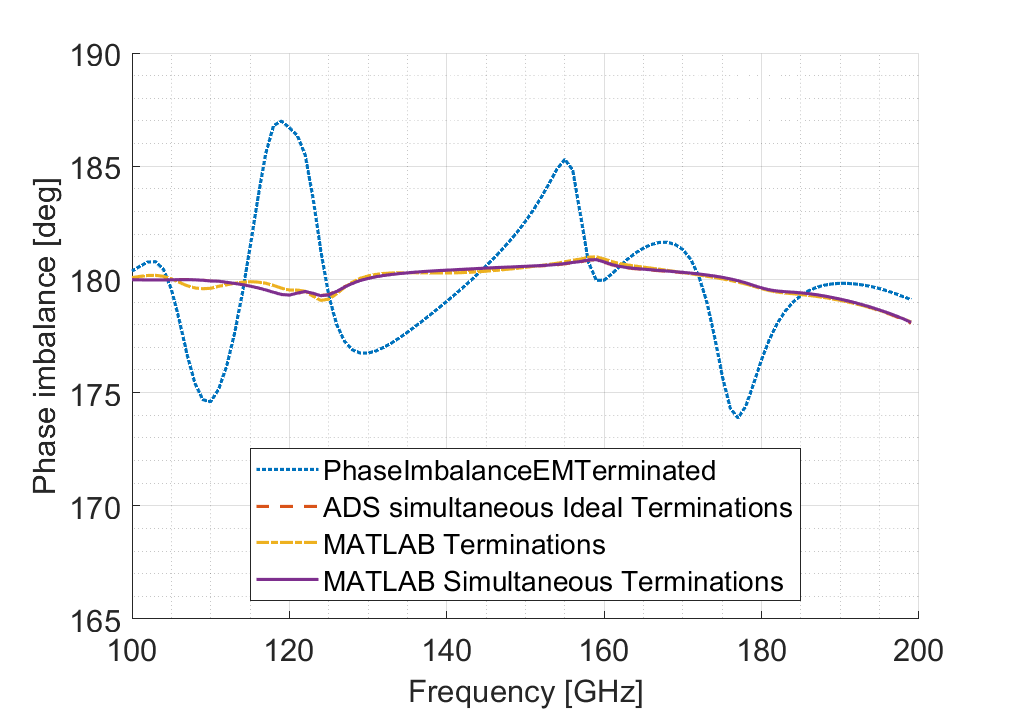
\includegraphics[width=\linewidth]{Design_figures/Layout/TapeoutMeasurements/FinalComparationPhaseImbalance_MatlabTermination.png}
    \end{subfigure}
    \caption{Caption}
    \label{fig:placeholder}
\end{figure}
\end{comment}

